\documentclass[11pt,a4paper]{article}

\usepackage[utf8]{inputenc}
\usepackage{graphicx}
\usepackage{float}
\usepackage[singlespacing]{setspace}
\usepackage[left=2.5cm,right=2.5cm,top=2cm,bottom=2cm]{geometry}
\usepackage{hyperref}

\setlength{\parskip}{5pt plus 1 pt minus 1 pt}

\begin{document}

\thispagestyle{empty}
\pagestyle{empty}

{\bf\centerline{{\huge Resume}}}
\vspace{6pt}

\centerline{Adrian Regenfuß (*28.10.1997)}
\centerline{Wriezener Straße 34}
\centerline{13359 Berlin, Germany}
\centerline{+49 177 6370390}
\centerline{adrian.regenfuss@posteo.de}
\centerline{\url{https://github.com/pranomostro}}
\smash{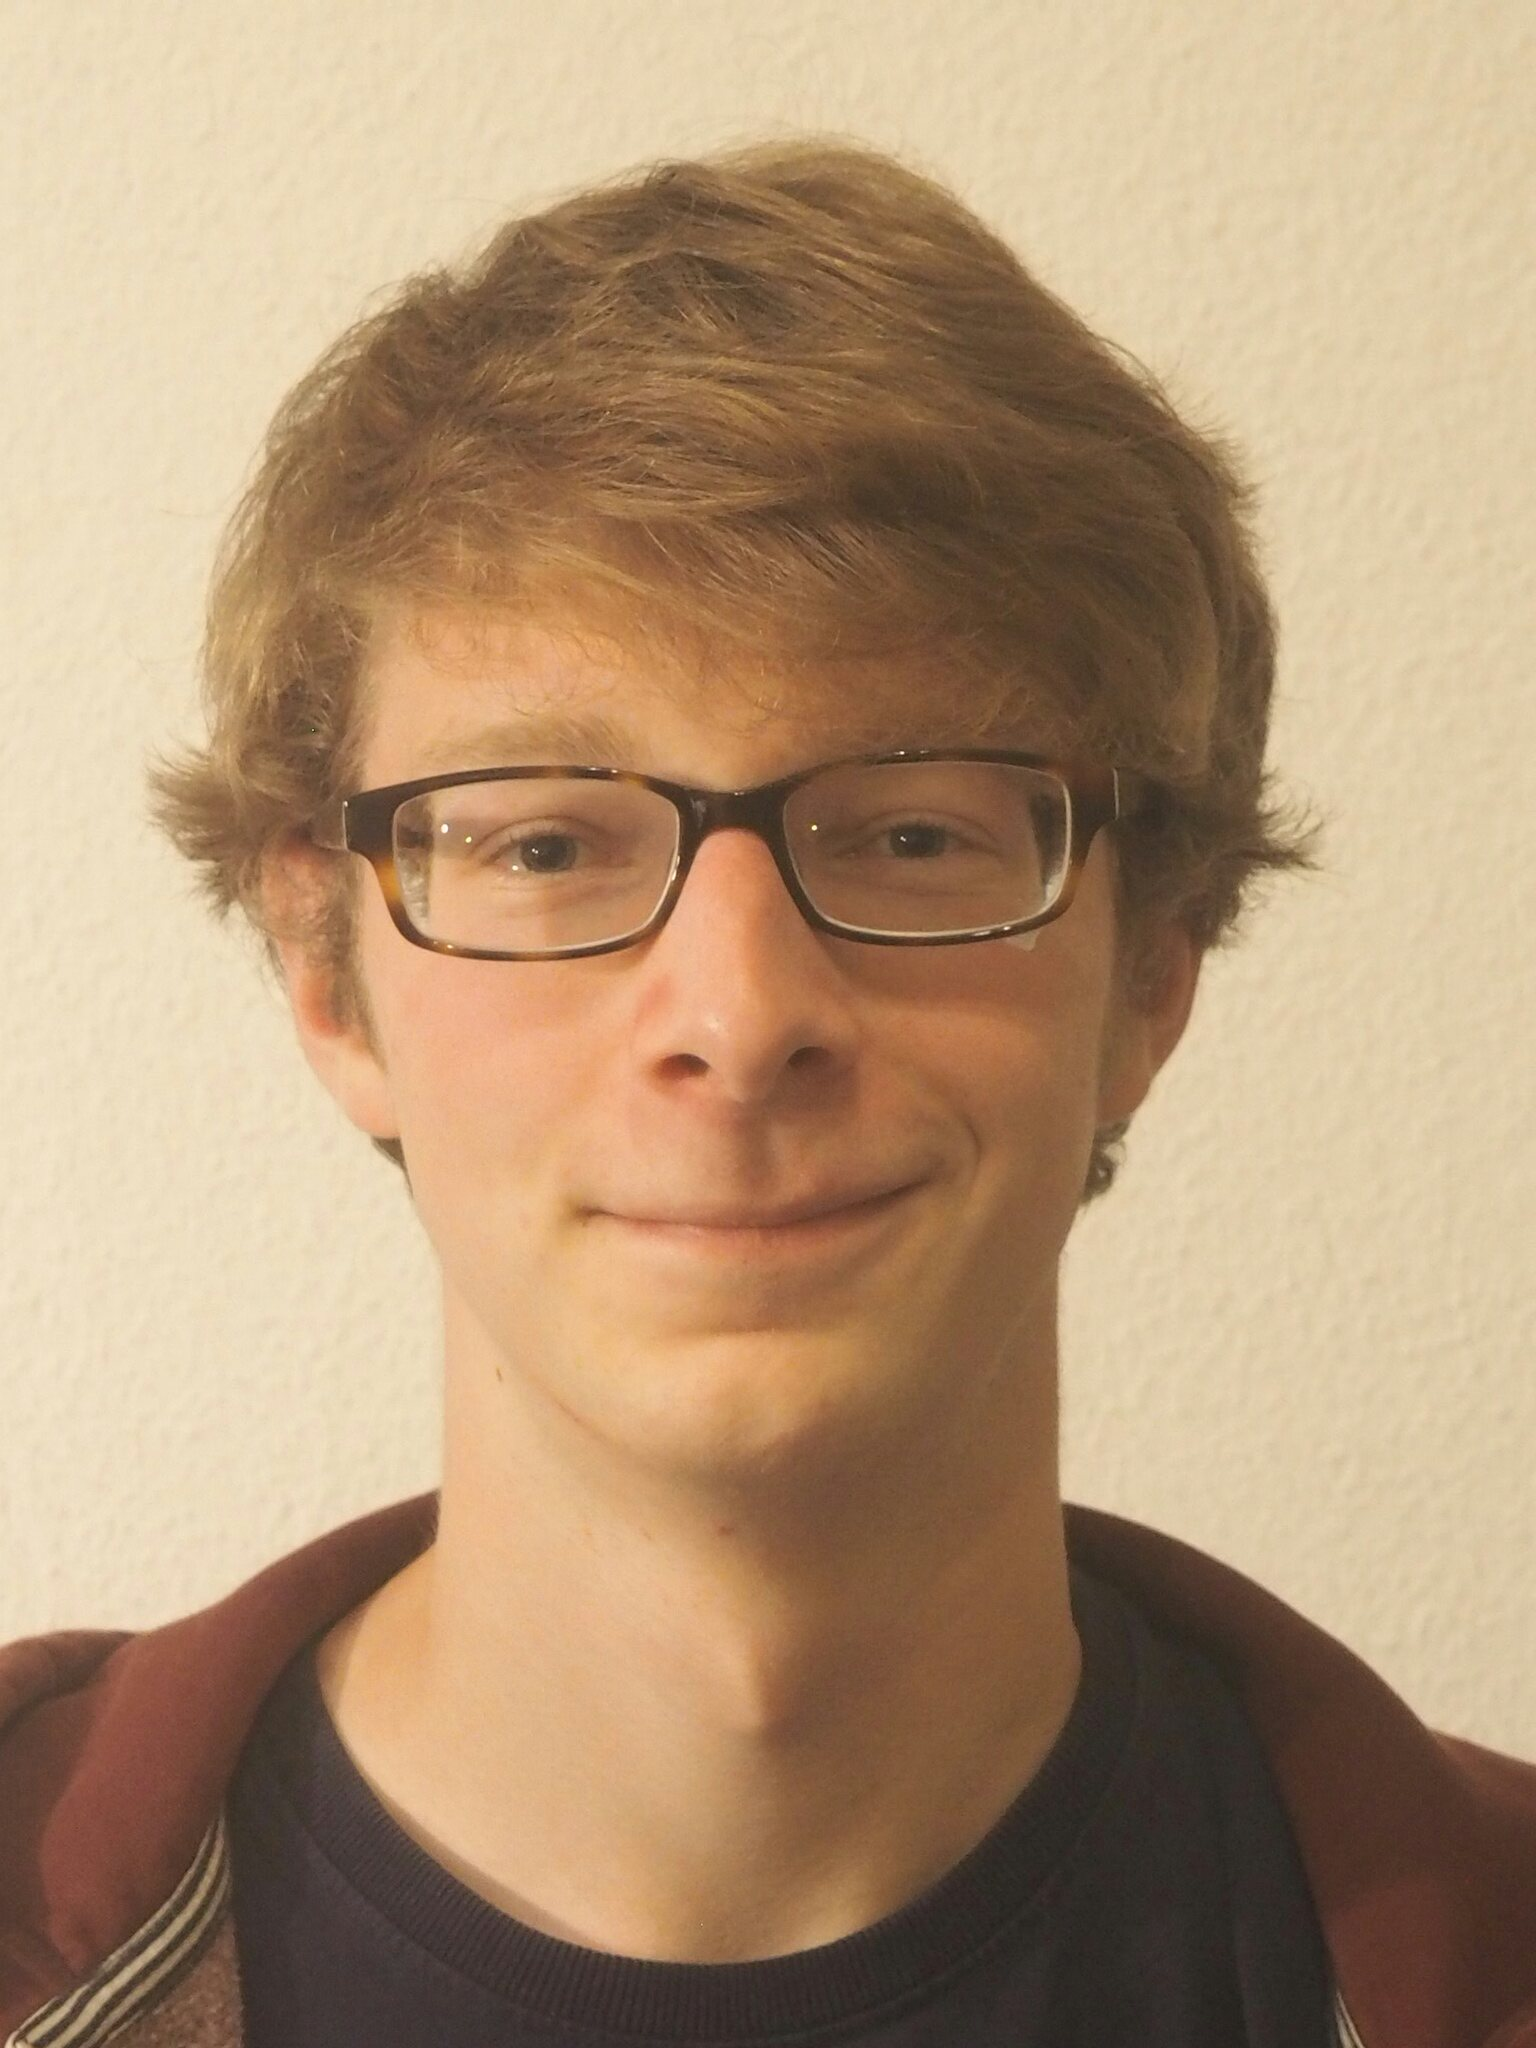
\includegraphics[scale=0.1]{./farbe.jpg}}

\section*{Education}
\begin{itemize}
	\setlength{\itemsep}{-2pt}
	\item Since April 2021: Computer Science at the Technical University of Berlin
	\item September 2017–March 2021: Computer Science at the Technical University of Munich
	\item Until June 2016: Highschool, finished with General Certificate of Education/GCE (German Abitur).
\end{itemize}

\vspace{-10pt}

\section*{Employment history}
\begin{itemize}
	\setlength{\itemsep}{-2pt}
	\item April 2020–April 2021: Part-time software developer at CQSE GmBH (www.cqse.eu), frontend development.
	\item May–September 2017: Internship at Bosch-Rexroth in Bangalore, India, writing an Android app for the superveillance of an engine control unit
	\item January-March 2017: Assembly line work at C. H. Beck printing presses
	\item September–November 2016: Internship at the Deep Learning Competence Center in the German Research Center for Artificial Intelligence
	(Deutsches Forschungszentrum für Künstliche Intelligenz, www.dfki.de), with focus on analysis of
	visual data using convolutional neural networks.
	\item June–July 2016: Summer job at Allocation Network GmbH in Munich (software maintenance and testing of a commercial supplier management system) \& eliminate duplicates in the companies exchange mail
	server database - design, build and test)
\end{itemize}

\vspace{-10pt}

\section*{Technical skills}
\begin{itemize}
	\setlength{\itemsep}{1pt}
	\item[]{\bf Languages}: C, Java, Lua, OCaml, SQL
	\item[]{\bf Web development}: Javascript, HTML, CSS, Typescript
	\item[]{\bf Tools}: git, make, gdb, awk, sed, regular expressions, LaTeX, Maven
\end{itemize}

\vspace{-10pt}

\section*{Extracurricular activities}
\begin{itemize}
	\setlength{\itemsep}{1pt}
	\item July 2016: Co-creation of an audio guide for a historic German labor camp near Munich
	\item July 2016–March 2021: Played in the protest band Beatprotest
	\item June 2019–March 2021: Co-organized Effective Altruism Munich
\end{itemize}

\vspace{-10pt}

\section*{References}
\begin{itemize}
	\item Daniel Veihelmann, Software Developer — CQSE GmbH Munich (veihelmann@cqse.eu)
	\item Andreas Vollmann, Director — Allocation Network GmbH Munich (mail@allocation.net)
\end{itemize}

\end{document}
